\title{Perry Williams}
\author{Ecologist and Statistician \\ Associate Professor \\ Department of Natural Resources and Environmental Science \\ University of Nevada, Reno}
\date{}

\maketitle

% --- Hero block: portrait + intro (image path must exist) ---
\begin{center}
\begin{minipage}{0.95\linewidth}
\begin{center}
  % Portrait on the left (CSS will make it round), text on the right
  % The CSS targets .hero and .portrait by structure, so this LaTeX just needs the image + paragraphs.
\end{center}
\end{minipage}
\end{center}

\begin{center}
  \begin{minipage}{0.95\linewidth}
  \vspace{-1.4em}
  \begin{center}
  \begin{tabular}{p{0.48\linewidth} p{0.44\linewidth}}
    \centering 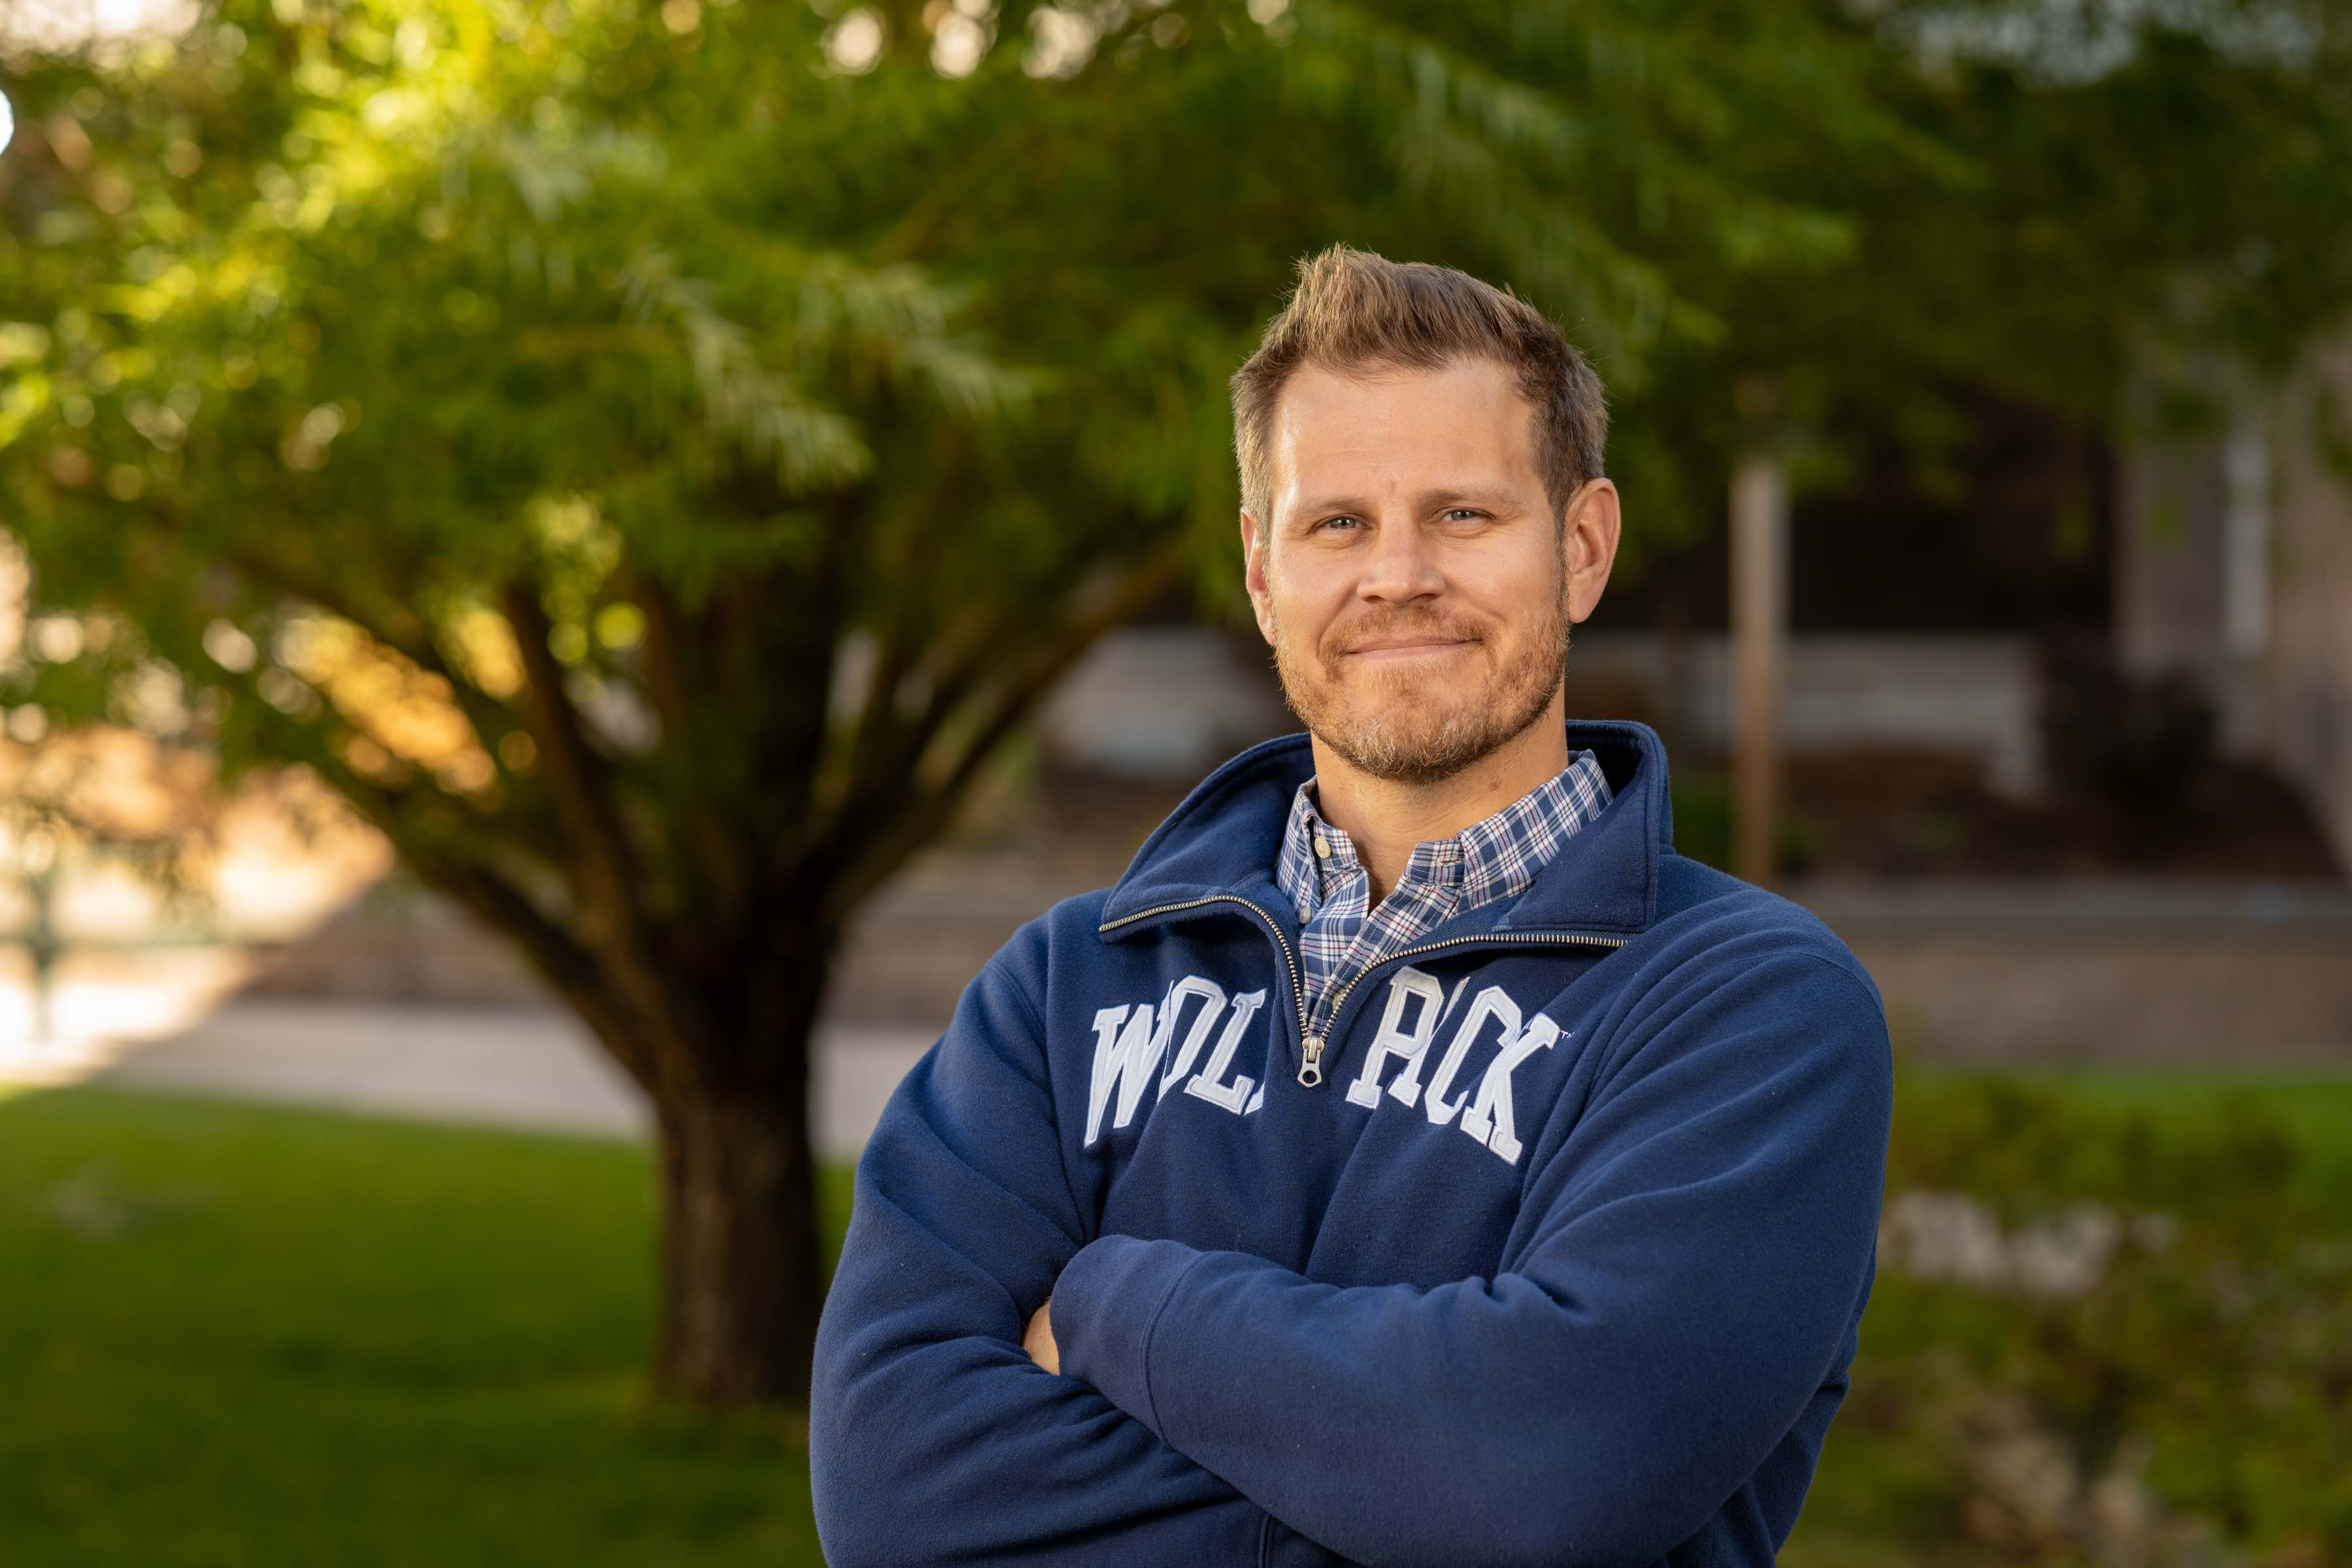
\includegraphics[width=0.70\linewidth]{assets/perry_2024.jpg} &

    \begin{minipage}{\linewidth}
      {\Large\textbf{Understanding patterns in the natural world}}\\[0.2em]
      \textit{Space, time, and uncertainty in ecological systems.}\\[0.6em]
      I study how populations and ecosystems change across space and time, with an emphasis on discovery and learning about complex natural processes. I build statistical and computational tools that advance ecological science and improve our ability to forecast environmental dynamics.\\[0.8em]

      \textbf{Contact:} \href{mailto:perryw@unr.edu}{perryw@unr.edu} \quad
      \textbf{GitHub:} \url{https://github.com/perrywilliamsunr}
      \\[0.6em]
      \noindent
      \fbox{\parbox{0.92\linewidth}{
        \textbf{Quick links:} \ \href{research.html}{Research} \quad|\quad \href{publications.html}{Publications} \quad|\quad \href{teaching.html}{Teaching} \quad|\quad \href{cv.html}{CV}
      }}
    \end{minipage}
  \end{tabular}
  \end{center}
  \end{minipage}
\end{center}

\section*{Highlights}
\begin{itemize}
  \item New tools for hierarchical Bayesian ecological diffusion to reveal how processes spread across landscapes.
  \item Generalizable case studies that connect species data to broader patterns in the natural environment.
  \item Reproducible workflows for forecasting and uncertainty quantification.
\end{itemize}

\section*{Current Projects}
\begin{itemize}
  \item \textbf{EcoDiffusion}: developing an R package for hierarchical Bayesian ecological diffusion models that help reveal how populations and processes spread across landscapes.
  \item Investigating population dynamics and movement (e.g., sage grouse) to understand large-scale ecological change.
  \item Exploring how human activities and natural variation shape species distributions (e.g., sea otters) as case studies of broader environmental patterns.
\end{itemize}
